\chapter{Secondo esercizio}

\section{GRASP}

\qs{}{Problema e soluzione di Creator}


\mypattern{Creator - Creatore}{
    \paragraph{Problema:} Chi crea un oggetto A? Chi deve essere responsabile
    della creazione di una nuova istanza di una classe?

    \paragraph{Soluzione:} Assegnare alla classe B la responsabilità di creare un'istanza della classe A 
    se una delle seguenti condizioni è vera:

    \begin{itemize}
        \item [$\Rightarrow$] B \textbf{aggrega} o \textbf{contiene} A;
        \item [$\Rightarrow$] B registra A\footnote{Registrare significa salvare un riferimento.};
        \item [$\Rightarrow$] B utilizza strettamente A;
        \item [$\Rightarrow$] B ha i dati necessari per inizializzare A.
    \end{itemize}
}

\qs{}{Problema e soluzione di Information Expert}

\mypattern{Information Expert - Esperto delle informazioni}{
    \paragraph{Problema:} Qual è un principio di base, generale, per l'assegnazione
    delle responsabilità agli oggetti?

    \paragraph{Soluzione:} Assegnare la responsabilità a un oggetto che ha le informazioni
    necessarie per soddisfarla, all’esperto delle informazioni, ovvero alla classe che possiede le
informazioni necessarie per soddisfare la responsabilita.
}

\qs{}{Problema e soluzione di Low Coupling}

\mypattern{Low Coupling - Accoppiamento basso}{
    \paragraph{Problema:} Come ridurre l’impatto dei cambiamenti? Come sostenere una dipendenza
    bassa, un impatto dei cambiamenti basso e una maggiore opportunità di riuso?

    \paragraph{Soluzione:} Assegnare le responsabilità in modo tale che l’accoppiamento (non necessario)
    rimanga basso.
}

\qs{}{Problema e soluzione di High Cohesion}

\mypattern{High Cohesion - Coesione alta}{
    \paragraph{Problema:} Come mantenere gli oggetti focalizzati, comprensibili e gestibili e, come effetto
    collaterale, sostenere Low Coupling?

    \paragraph{Soluzione:} Assegnare le responsabilità in modo tale che la coesione rimanga alta.

}

\qs{}{Problema e soluzione di Controller}

\mypattern{Controller - Controllore}{
    \paragraph{Problema:} Qual è il primo oggetto oltre lo strato UI che riceve e coordina (“controlla”)
    un’operazione di sistema?

    \paragraph{Soluzione:} Assegnare le responsabilità a un oggetto che rappresenta una delle seguenti scelte:
    \begin{itemize}
        \item [$\Rightarrow$] Un oggetto che rappresenta il sistema (facede controller);
        \item [$\Rightarrow$] Un oggetto che rappresenta uno scenario di un Caso d’Uso
        (controller di Caso d'Uso o controller di sessione).
    \end{itemize}
}

\section{GoF}
\subsection{Decorator}
\begin{center}
  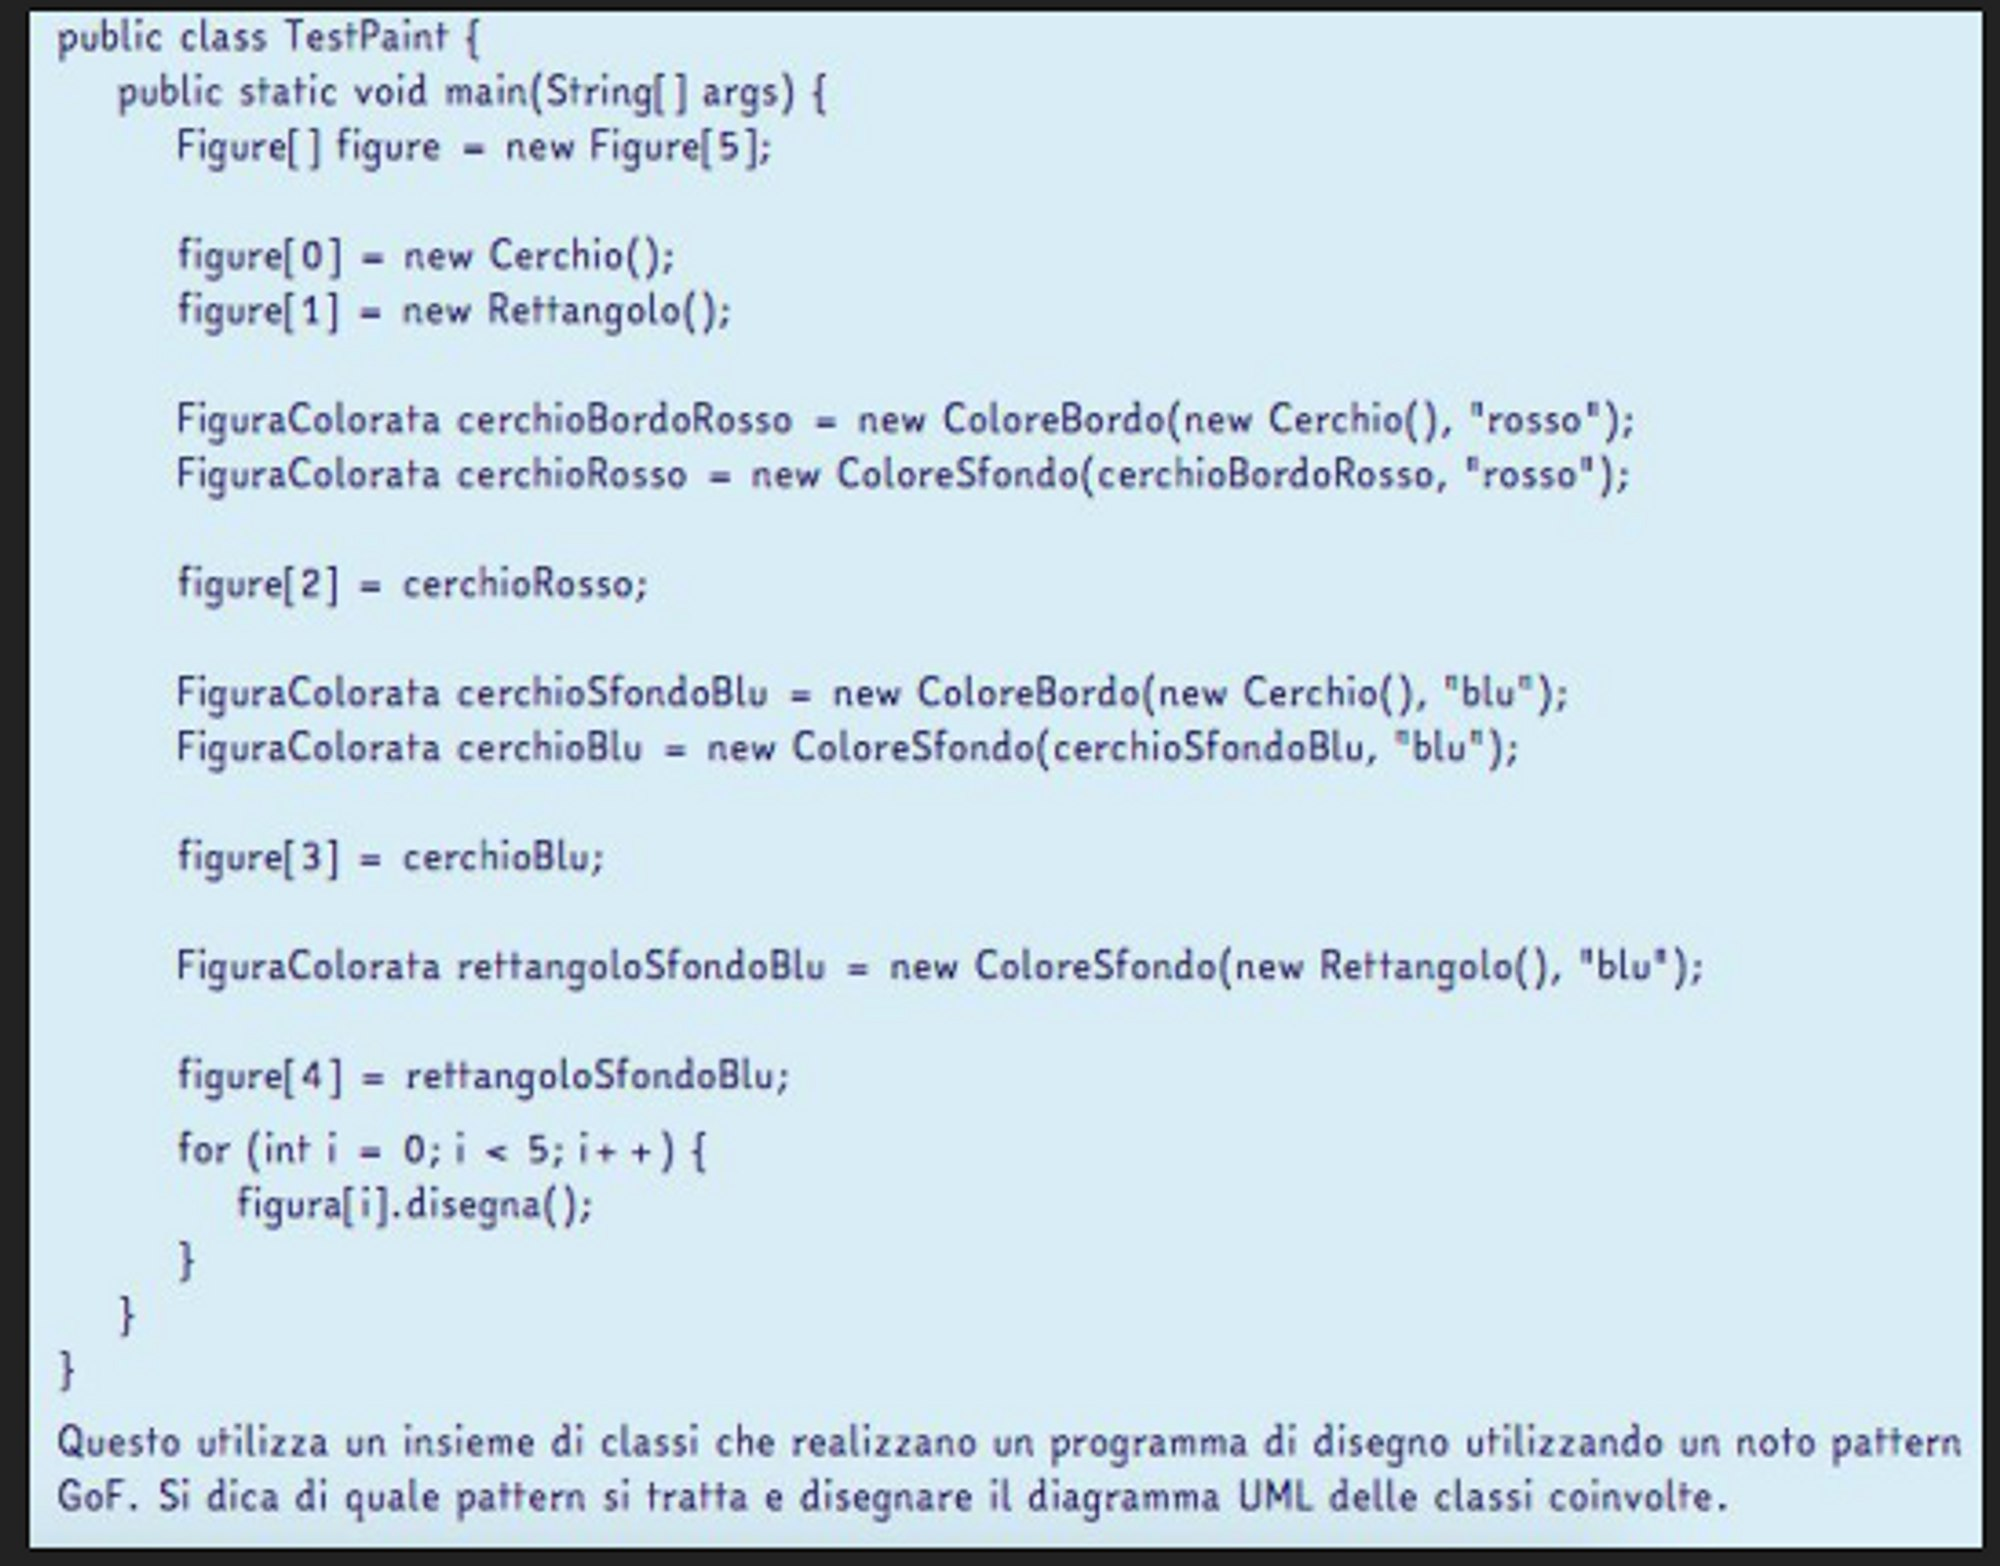
\includegraphics[scale=0.2]{GoF/Decorator.jpg}
\end{center}

\nt{Quando vengono aggiunte nuove funzionalità, di solito è Decorator}

\begin{center}
  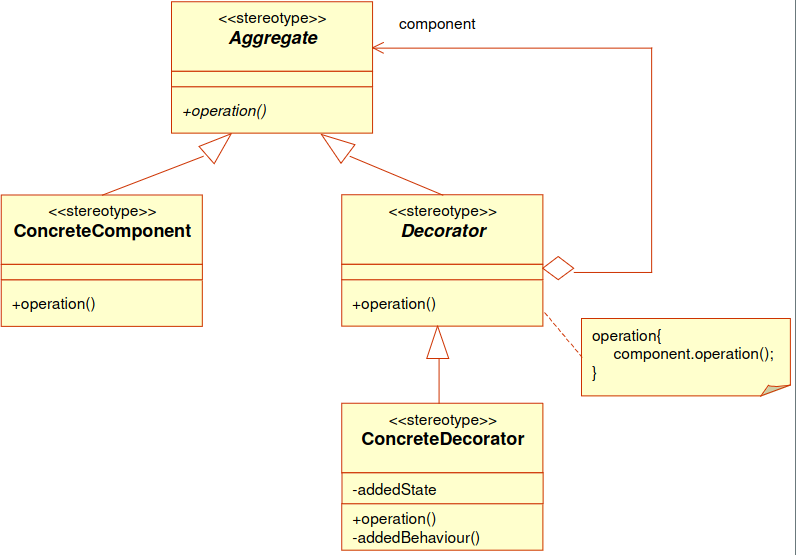
\includegraphics[scale=0.5]{GoF/Decorator.png}
\end{center}

\pagebreak
\subsection{Composite}
\begin{center}
  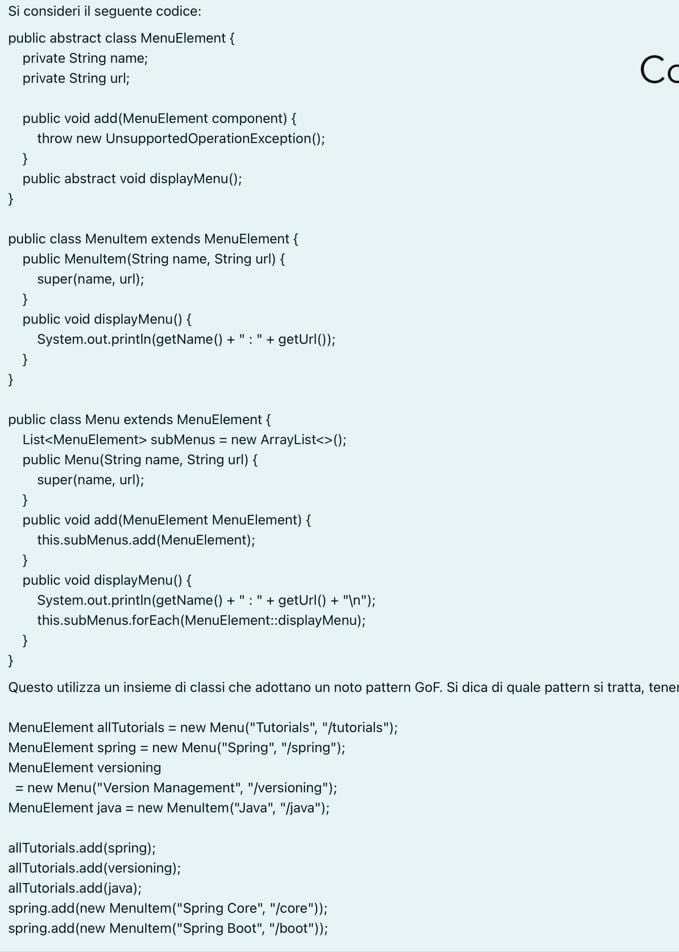
\includegraphics[scale=0.35]{GoF/Composite.jpg}
\end{center}

\nt{Generalmente i Composite sono alberi o strutture ricorsive. In questo caso si può notare che sia \texttt{Menu} che \texttt{MenuItem} implementano il displayMenu(), ma è possibile aggiungere nuovi elementi solo al Composto (\texttt{Menu}). Se si tenta di aggiungere nuovi elementi a \texttt{MenuItem}, non essendo ridefinito add(component: \texttt{MenuElement}) viene utilizzato il metodo della classe astratta \texttt{MenuElement} che lancia un'eccezione.}

\begin{center}
  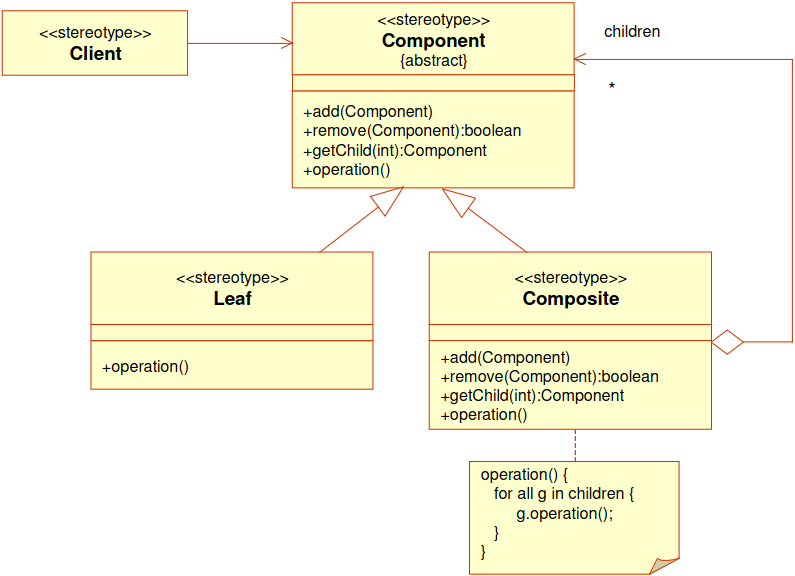
\includegraphics[scale=0.6]{GoF/Composite.png}
\end{center}

\pagebreak

\subsection{Strategy}

\begin{center}
  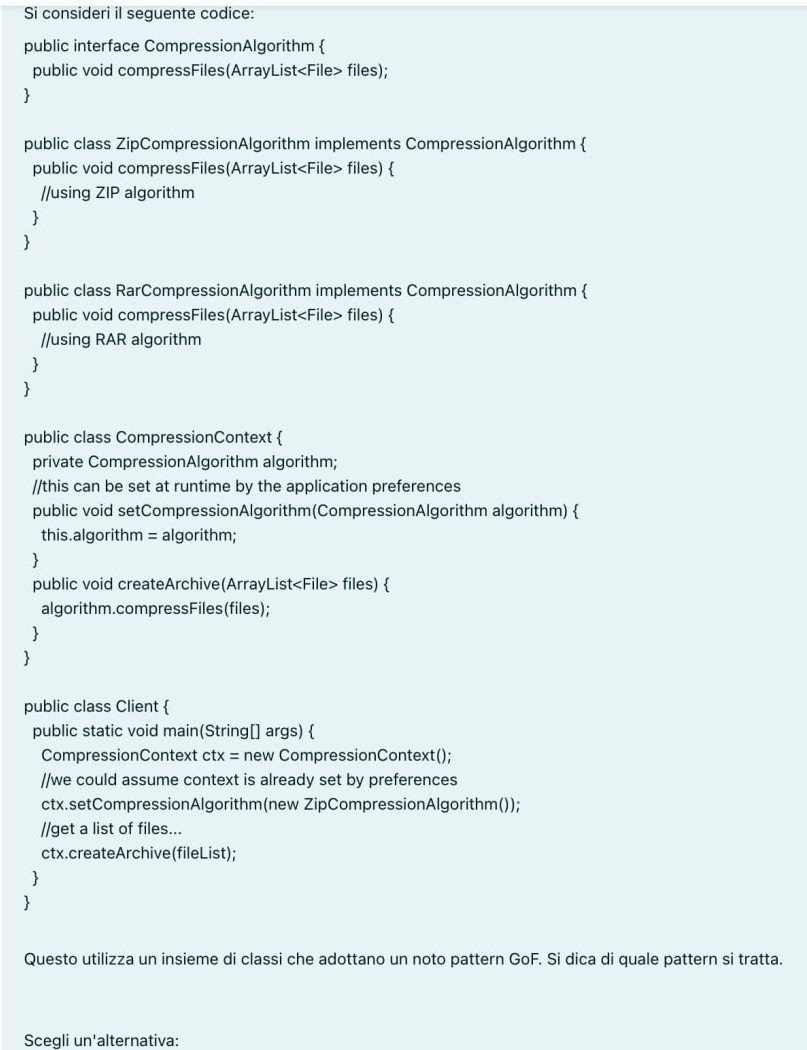
\includegraphics[scale=0.4]{GoF/Strategy.jpg}
\end{center}

\nt{Strategy viene utilizzato quando ci sono più possibilità tra cui scegliere. Per esempio tra diversi algoritmi (di ordinamento, compressione, etc.) che fanno tutti la stessa cosa, ma in modo diverso.}

\begin{center}
  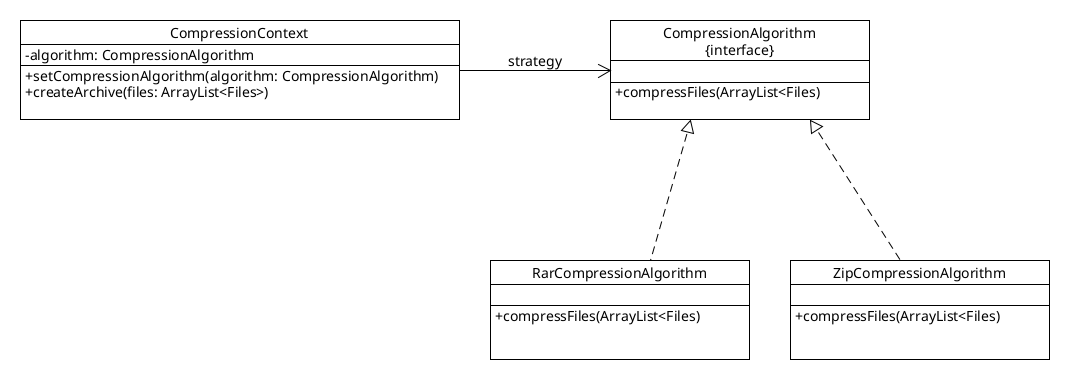
\includegraphics[scale=0.45]{GoF/Strategy.png}
\end{center}

\subsection{Visitor}

\begin{center}
  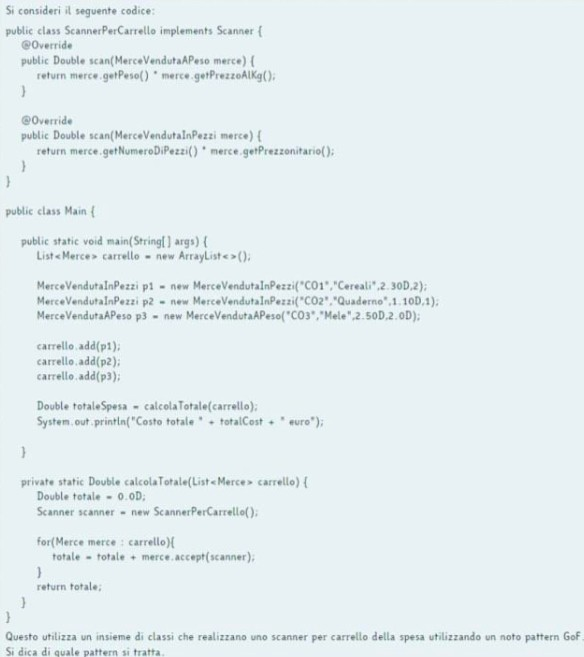
\includegraphics[scale=0.7]{GoF/Visitor.jpg}
\end{center}

\nt{Visitor lo si ha quando si tenta di effettuare un'operazione (in questo caso un calcolo) su elementi che possono essere diversi e devono essere trattati in modo diverso (in questo caso \texttt{MerceVendutaInPezzi} e \texttt{MerceVendutaAPeso}).}

\begin{center}
  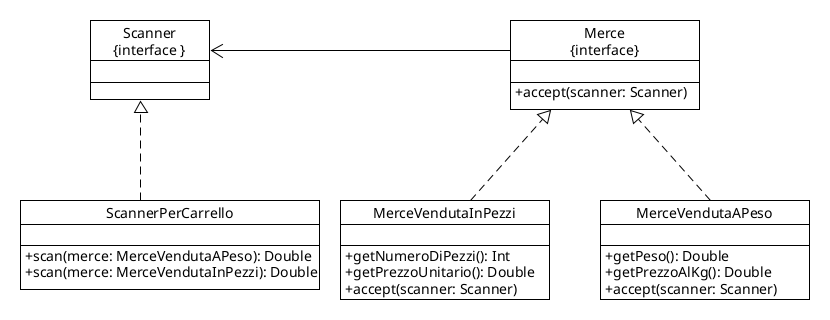
\includegraphics[scale=0.55]{GoF/Visitor.png}
\end{center}

\pagebreak

\subsection{State}

\begin{center}
  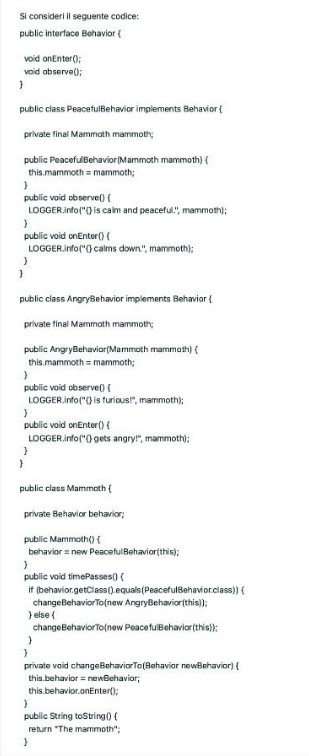
\includegraphics[scale=0.65]{GoF/State.jpg}
\end{center}

\nt{State si riconosce dal fatto che c'è sempre un "pulsante" per cambiare stato. In questo esempio lo stato cambia a seconda della nuova \texttt{Behavior} passata, ma può capitare che lo stato si alterni tra 2 o 3 valori senza necessità di passare esplicitamente un parametro.}

\begin{center}
  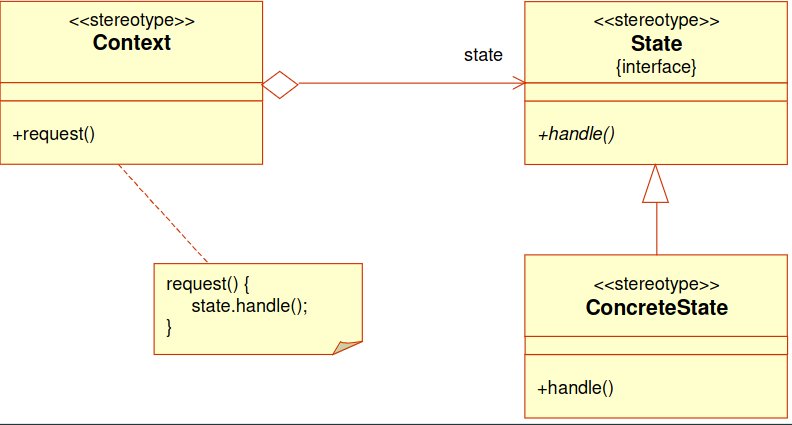
\includegraphics[scale=0.6]{GoF/State.png}
\end{center}

\pagebreak 

\subsection{Observer}

\begin{center}
  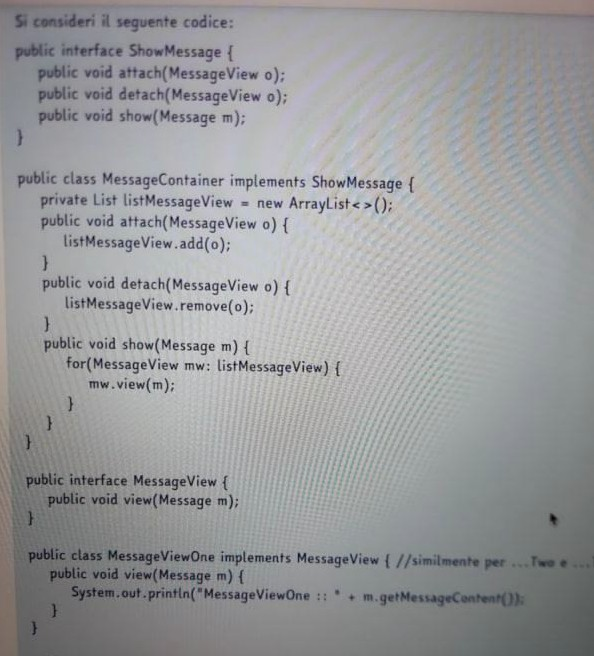
\includegraphics[scale=0.65]{GoF/Observer.jpg}
\end{center}

\nt{Observer ha sempre un metodo per attaccarsi/iscriversi e uno per staccarsi/disiscriversi. Inoltre hanno anche un metodo per notificare gli osservatori (in questo caso show(m: \texttt{Message})).}

\begin{center}
  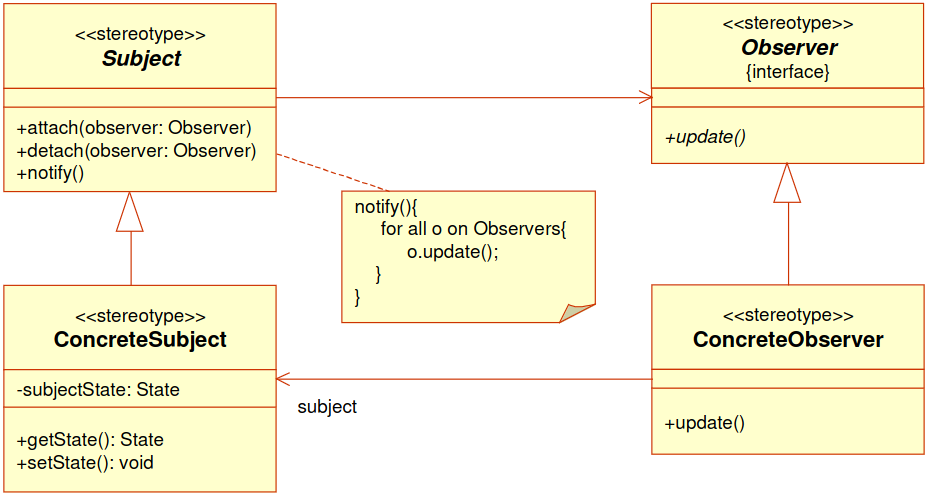
\includegraphics[scale=0.6]{GoF/Observer.png}
\end{center}

\pagebreak

\subsection{Adapter}

\begin{center}
  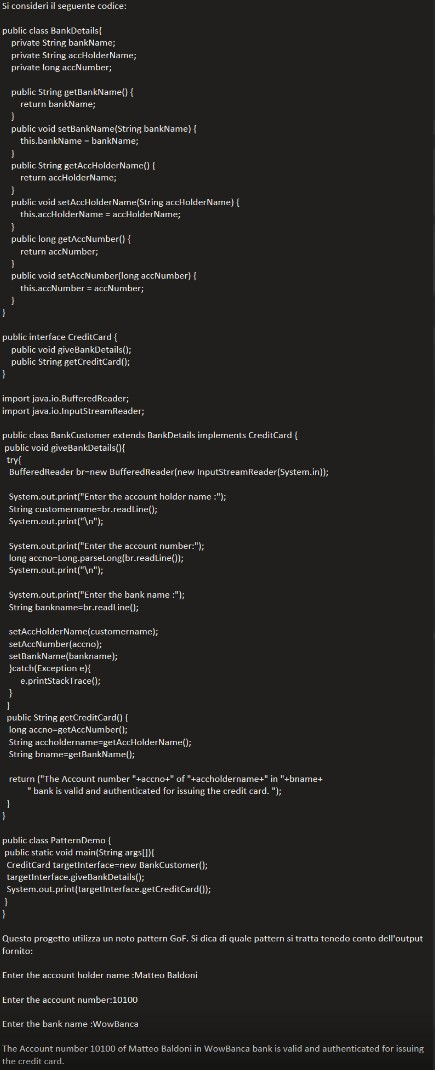
\includegraphics[scale=0.8]{GoF/Adapter.jpg}
\end{center}

\nt{Adapter è abbastanza riconoscibile, ma bisogna stare attenti a quale versione viene messa. Probabilmente se uscirà sarà la versione "oggetto" perché è migliore rispetto alla versione "classe". Ma nulla vieta ai prof. di mettere quest'ultima.}

\begin{center}
  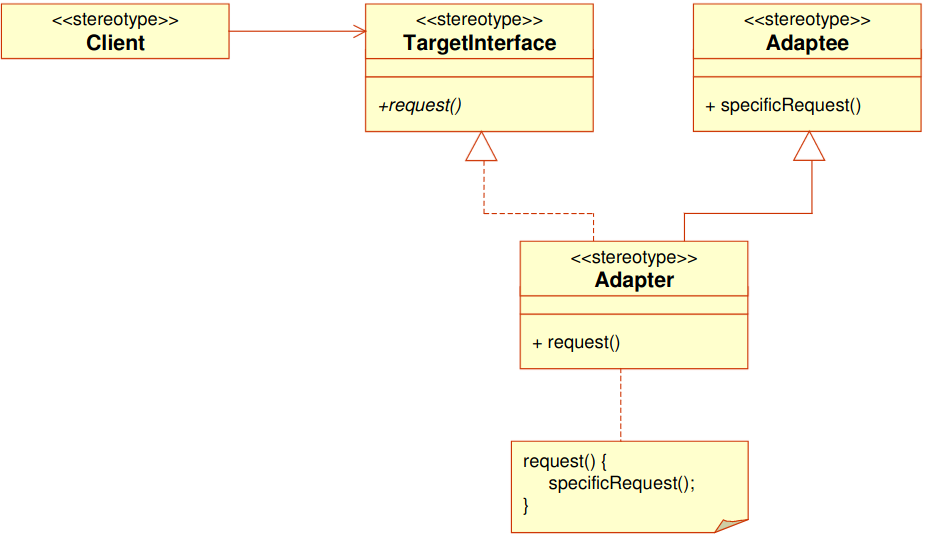
\includegraphics[scale=0.7]{GoF/Adapter.png}
\end{center}

\subsection{AbstractFactory e Singleton}

\nt{Singleton è facilmente riconoscibile dal fatto che può apparire come classe statica o con un metodo che restituisce la sua istanza se non è null o una nuova istanza se è null.}

\nt{AbstractFactory è evidente dal fatto che viene usato per creare oggetti e non è il Singleton.}


